\cleardoublepage
\chapter{Diskusjon}
\label{chap:discussion} 

I dette kapittelet vil resultatet bli diskutert. Kapittelet vil fokusere på om resultatet ble som forventet, om oppdragsgiver var fornøyd med resultatet, om gruppen gjort noe annerledes/bedre og hva gruppen har lært underveis. Det vil også inneholde en vurdering av produktet opp mot relatert arbeid. Gruppen vil gi anbefalinger og fremlegge designprinsipper for videre arbeid og utvikling av plattformen i praksis. Til slutt er en konklusjon med oppsummering av arbeidet og prosessen.

\section{Resultat i forhold til oppdragsgivers forventinger}

\section{Resultat i forhold til sluttbrukerens krav}

\section{Gruppens evaluering}

\section{Vurdering av produkt opp mot relatert arbeid}

\section{Erfaringer gjort underveis}
\subsection{Hva kunne blitt gjort annerledes?}

\section{Anbefalinger for utvikling og videre arbeid}
\subsection{Database}
Siden systemet inkluderer innlogging og informasjon fra andre kilder enn Brønnøysundregisteret er det behov for en database som lagrer passord, brukernavn og øvrig info om både brukere, organisasjoner og administrator. Figur~\ref{fig:databasemodell} viser en modell av informasjonen som lagres i databasen.

Koblingene mellom tabellene viser til at hver organisasjon kan ha flere brukerprofiler tilknyttet seg, samtidig som hver bruker kan være tilknyttet flere organisasjoner. Hver bruker kan også være tilknyttet flere andre brukere.

Inkludert i systemet er et administratorpanel der så mye som mulig er automatisert i systemet, slik at det ikke trengs mer enn 5-10 minutter per uke med vedlikehold fra administrator sin side.
\\
\begin{figure}[H]
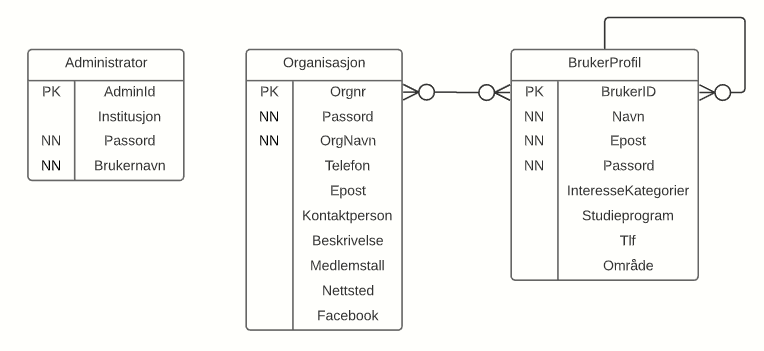
\includegraphics[width=\textwidth]{Illustrasjoner/databasemodell-2.png}
\caption{Databasemodell for lagring av informasjon for Administrator, Organisasjon og Brukerprofil}
\label{fig:databasemodell}
\end{figure}

\subsection{Feide og tilgang til studentinformasjon}

\subsection{Merkevarebygging og synliggjøring av produktet}

Produktet blir laget i samkoordinering med Høgskolen i Østfold som et av deres bachelorprosjekter. Dette alene gir stor vekt blant aktører og organisasjoner som vil kunne være interessert i et slikt produkt, enda mer om Høgskolen i Østfold offentlig stiller seg bak produktet og bruker det som en del av sin hjemmeside.

Utfordringen blir å skape et levende produkt, hvor organisasjoner legger inn egen informasjon og sørger for at ny og oppdatert informasjon blir lagt til kontinuerlig. Dette innebærer at det må være attraktivt for organisasjoner og legge til informasjon og oppdatere sine sider inne på plattformen.

\paragraph{Hvordan kan dette løses?}

Produktet må være godt synlig og lett tilgjengelig plassert på fremsiden til Høgskolen i Østfold for at dette produktet skal bli brukt av studenter. det anbefalles også at det blir kjørt et redesign av HIØ sitt nettsted ettersom det er ganske kaotisk på nåværende tidspunkt. For at det skal være attraktivt for organisasjoner å legge inn og oppdatere sin informasjon så skal det introduseres ett system som plasserer organisasjoner med oppdatert informasjon lengre opp på resultat listene. I tillegg skal det i start fasen av produktet kontaktes en del store organisasjoner for å få de til å legge til informasjon om seg selv som igjen kan starte et initiativ hos andre til å legge til sin informasjon. 

\paragraph{Videre markedsføring og fremtidsplan for produktet}

Dette produktet blir bygget i hovedsak for HIØ. Men det betyr ikke at produktet kun begrenses til kommunene Fredrikstad, Sarpsborg og Halden. Informasjonen som hentes ut fra brreg.no dekker hele Norge. Det betyr at systemet har tilgang på all den informasjonen og ved noen enkle endringer på område parameterene i programmet til produktet kan det tilbys til for eksempel andre høyskoler, kommuner, fylker og interesserte parter. Det vil si at produktet kan da tilbys til andre nettsteder, som vil skape et større navn for vår merkevare. dette er med på å få de forskjellige organisasjonene til å se på det som attraktivt å legge inn sin informasjon som vil skape en god sirkel av merkevarebygging for alle parter. 


\section{Konklusjon og oppsummering}







